% Options for packages loaded elsewhere
\PassOptionsToPackage{unicode}{hyperref}
\PassOptionsToPackage{hyphens}{url}
%
\documentclass[
]{article}
\usepackage{amsmath,amssymb}
\usepackage{iftex}
\ifPDFTeX
  \usepackage[T1]{fontenc}
  \usepackage[utf8]{inputenc}
  \usepackage{textcomp} % provide euro and other symbols
\else % if luatex or xetex
  \usepackage{unicode-math} % this also loads fontspec
  \defaultfontfeatures{Scale=MatchLowercase}
  \defaultfontfeatures[\rmfamily]{Ligatures=TeX,Scale=1}
\fi
\usepackage{lmodern}
\ifPDFTeX\else
  % xetex/luatex font selection
\fi
% Use upquote if available, for straight quotes in verbatim environments
\IfFileExists{upquote.sty}{\usepackage{upquote}}{}
\IfFileExists{microtype.sty}{% use microtype if available
  \usepackage[]{microtype}
  \UseMicrotypeSet[protrusion]{basicmath} % disable protrusion for tt fonts
}{}
\makeatletter
\@ifundefined{KOMAClassName}{% if non-KOMA class
  \IfFileExists{parskip.sty}{%
    \usepackage{parskip}
  }{% else
    \setlength{\parindent}{0pt}
    \setlength{\parskip}{6pt plus 2pt minus 1pt}}
}{% if KOMA class
  \KOMAoptions{parskip=half}}
\makeatother
\usepackage{xcolor}
\usepackage[margin=1in]{geometry}
\usepackage{color}
\usepackage{fancyvrb}
\newcommand{\VerbBar}{|}
\newcommand{\VERB}{\Verb[commandchars=\\\{\}]}
\DefineVerbatimEnvironment{Highlighting}{Verbatim}{commandchars=\\\{\}}
% Add ',fontsize=\small' for more characters per line
\usepackage{framed}
\definecolor{shadecolor}{RGB}{248,248,248}
\newenvironment{Shaded}{\begin{snugshade}}{\end{snugshade}}
\newcommand{\AlertTok}[1]{\textcolor[rgb]{0.94,0.16,0.16}{#1}}
\newcommand{\AnnotationTok}[1]{\textcolor[rgb]{0.56,0.35,0.01}{\textbf{\textit{#1}}}}
\newcommand{\AttributeTok}[1]{\textcolor[rgb]{0.13,0.29,0.53}{#1}}
\newcommand{\BaseNTok}[1]{\textcolor[rgb]{0.00,0.00,0.81}{#1}}
\newcommand{\BuiltInTok}[1]{#1}
\newcommand{\CharTok}[1]{\textcolor[rgb]{0.31,0.60,0.02}{#1}}
\newcommand{\CommentTok}[1]{\textcolor[rgb]{0.56,0.35,0.01}{\textit{#1}}}
\newcommand{\CommentVarTok}[1]{\textcolor[rgb]{0.56,0.35,0.01}{\textbf{\textit{#1}}}}
\newcommand{\ConstantTok}[1]{\textcolor[rgb]{0.56,0.35,0.01}{#1}}
\newcommand{\ControlFlowTok}[1]{\textcolor[rgb]{0.13,0.29,0.53}{\textbf{#1}}}
\newcommand{\DataTypeTok}[1]{\textcolor[rgb]{0.13,0.29,0.53}{#1}}
\newcommand{\DecValTok}[1]{\textcolor[rgb]{0.00,0.00,0.81}{#1}}
\newcommand{\DocumentationTok}[1]{\textcolor[rgb]{0.56,0.35,0.01}{\textbf{\textit{#1}}}}
\newcommand{\ErrorTok}[1]{\textcolor[rgb]{0.64,0.00,0.00}{\textbf{#1}}}
\newcommand{\ExtensionTok}[1]{#1}
\newcommand{\FloatTok}[1]{\textcolor[rgb]{0.00,0.00,0.81}{#1}}
\newcommand{\FunctionTok}[1]{\textcolor[rgb]{0.13,0.29,0.53}{\textbf{#1}}}
\newcommand{\ImportTok}[1]{#1}
\newcommand{\InformationTok}[1]{\textcolor[rgb]{0.56,0.35,0.01}{\textbf{\textit{#1}}}}
\newcommand{\KeywordTok}[1]{\textcolor[rgb]{0.13,0.29,0.53}{\textbf{#1}}}
\newcommand{\NormalTok}[1]{#1}
\newcommand{\OperatorTok}[1]{\textcolor[rgb]{0.81,0.36,0.00}{\textbf{#1}}}
\newcommand{\OtherTok}[1]{\textcolor[rgb]{0.56,0.35,0.01}{#1}}
\newcommand{\PreprocessorTok}[1]{\textcolor[rgb]{0.56,0.35,0.01}{\textit{#1}}}
\newcommand{\RegionMarkerTok}[1]{#1}
\newcommand{\SpecialCharTok}[1]{\textcolor[rgb]{0.81,0.36,0.00}{\textbf{#1}}}
\newcommand{\SpecialStringTok}[1]{\textcolor[rgb]{0.31,0.60,0.02}{#1}}
\newcommand{\StringTok}[1]{\textcolor[rgb]{0.31,0.60,0.02}{#1}}
\newcommand{\VariableTok}[1]{\textcolor[rgb]{0.00,0.00,0.00}{#1}}
\newcommand{\VerbatimStringTok}[1]{\textcolor[rgb]{0.31,0.60,0.02}{#1}}
\newcommand{\WarningTok}[1]{\textcolor[rgb]{0.56,0.35,0.01}{\textbf{\textit{#1}}}}
\usepackage{graphicx}
\makeatletter
\def\maxwidth{\ifdim\Gin@nat@width>\linewidth\linewidth\else\Gin@nat@width\fi}
\def\maxheight{\ifdim\Gin@nat@height>\textheight\textheight\else\Gin@nat@height\fi}
\makeatother
% Scale images if necessary, so that they will not overflow the page
% margins by default, and it is still possible to overwrite the defaults
% using explicit options in \includegraphics[width, height, ...]{}
\setkeys{Gin}{width=\maxwidth,height=\maxheight,keepaspectratio}
% Set default figure placement to htbp
\makeatletter
\def\fps@figure{htbp}
\makeatother
\setlength{\emergencystretch}{3em} % prevent overfull lines
\providecommand{\tightlist}{%
  \setlength{\itemsep}{0pt}\setlength{\parskip}{0pt}}
\setcounter{secnumdepth}{-\maxdimen} % remove section numbering
\ifLuaTeX
  \usepackage{selnolig}  % disable illegal ligatures
\fi
\IfFileExists{bookmark.sty}{\usepackage{bookmark}}{\usepackage{hyperref}}
\IfFileExists{xurl.sty}{\usepackage{xurl}}{} % add URL line breaks if available
\urlstyle{same}
\hypersetup{
  pdftitle={LDA\_QDA\_Example},
  pdfauthor={STAT380},
  hidelinks,
  pdfcreator={LaTeX via pandoc}}

\title{LDA\_QDA\_Example}
\author{STAT380}
\date{2023-10-12}

\begin{document}
\maketitle

\hypertarget{loading-the-iris-data}{%
\section{Loading the Iris Data}\label{loading-the-iris-data}}

\begin{Shaded}
\begin{Highlighting}[]
\DocumentationTok{\#\#\# Example 1: Iris data}
\FunctionTok{library}\NormalTok{(MASS)}
\FunctionTok{library}\NormalTok{(ggplot2)}
\FunctionTok{data}\NormalTok{(}\StringTok{"iris"}\NormalTok{)}
\FunctionTok{str}\NormalTok{(iris)}
\end{Highlighting}
\end{Shaded}

\begin{verbatim}
## 'data.frame':    150 obs. of  5 variables:
##  $ Sepal.Length: num  5.1 4.9 4.7 4.6 5 5.4 4.6 5 4.4 4.9 ...
##  $ Sepal.Width : num  3.5 3 3.2 3.1 3.6 3.9 3.4 3.4 2.9 3.1 ...
##  $ Petal.Length: num  1.4 1.4 1.3 1.5 1.4 1.7 1.4 1.5 1.4 1.5 ...
##  $ Petal.Width : num  0.2 0.2 0.2 0.2 0.2 0.4 0.3 0.2 0.2 0.1 ...
##  $ Species     : Factor w/ 3 levels "setosa","versicolor",..: 1 1 1 1 1 1 1 1 1 1 ...
\end{verbatim}

\begin{Shaded}
\begin{Highlighting}[]
\FunctionTok{head}\NormalTok{(iris)}
\end{Highlighting}
\end{Shaded}

\begin{verbatim}
##   Sepal.Length Sepal.Width Petal.Length Petal.Width Species
## 1          5.1         3.5          1.4         0.2  setosa
## 2          4.9         3.0          1.4         0.2  setosa
## 3          4.7         3.2          1.3         0.2  setosa
## 4          4.6         3.1          1.5         0.2  setosa
## 5          5.0         3.6          1.4         0.2  setosa
## 6          5.4         3.9          1.7         0.4  setosa
\end{verbatim}

\hypertarget{basic-plots-to-see-the-interrelation-between-the-variables}{%
\section{Basic plots to see the interrelation between the
variables}\label{basic-plots-to-see-the-interrelation-between-the-variables}}

\begin{Shaded}
\begin{Highlighting}[]
\FunctionTok{pairs}\NormalTok{(iris[}\DecValTok{1}\SpecialCharTok{:}\DecValTok{4}\NormalTok{],}
             \AttributeTok{gap =} \DecValTok{0}\NormalTok{,}
             \AttributeTok{bg =} \FunctionTok{c}\NormalTok{(}\StringTok{"red"}\NormalTok{, }\StringTok{"green"}\NormalTok{, }\StringTok{"blue"}\NormalTok{)[iris}\SpecialCharTok{$}\NormalTok{Species],}
             \AttributeTok{pch =} \DecValTok{21}\NormalTok{)}
\end{Highlighting}
\end{Shaded}

\includegraphics{LDA_QDA_IRIS_files/figure-latex/unnamed-chunk-1-1.pdf}

\hypertarget{splitting-the-data-in-training-and-testing-set}{%
\section{Splitting the Data in Training and Testing
Set}\label{splitting-the-data-in-training-and-testing-set}}

\begin{Shaded}
\begin{Highlighting}[]
\FunctionTok{set.seed}\NormalTok{(}\DecValTok{134}\NormalTok{)}
\NormalTok{ind }\OtherTok{=} \FunctionTok{sample}\NormalTok{(}\DecValTok{2}\NormalTok{, }\FunctionTok{nrow}\NormalTok{(iris), }\AttributeTok{replace =} \ConstantTok{TRUE}\NormalTok{, }\AttributeTok{prob =} \FunctionTok{c}\NormalTok{(}\FloatTok{0.6}\NormalTok{, }\FloatTok{0.4}\NormalTok{))}
\NormalTok{training }\OtherTok{=}\NormalTok{ iris[ind}\SpecialCharTok{==}\DecValTok{1}\NormalTok{,]}
\NormalTok{testing }\OtherTok{=}\NormalTok{ iris[ind}\SpecialCharTok{==}\DecValTok{2}\NormalTok{,]}
\end{Highlighting}
\end{Shaded}

\hypertarget{fitting-a-linear-discriminant-analysis}{%
\section{Fitting a Linear Discriminant
Analysis}\label{fitting-a-linear-discriminant-analysis}}

\begin{Shaded}
\begin{Highlighting}[]
\NormalTok{iris\_lda }\OtherTok{=} \FunctionTok{lda}\NormalTok{(Species}\SpecialCharTok{\textasciitilde{}}\NormalTok{., training)}
\NormalTok{iris\_lda}
\end{Highlighting}
\end{Shaded}

\begin{verbatim}
## Call:
## lda(Species ~ ., data = training)
## 
## Prior probabilities of groups:
##     setosa versicolor  virginica 
##  0.3367347  0.3469388  0.3163265 
## 
## Group means:
##            Sepal.Length Sepal.Width Petal.Length Petal.Width
## setosa         5.006061    3.457576     1.439394   0.2575758
## versicolor     5.932353    2.735294     4.223529   1.3147059
## virginica      6.438710    2.935484     5.445161   1.9774194
## 
## Coefficients of linear discriminants:
##                     LD1        LD2
## Sepal.Length  0.9583651 -0.6656007
## Sepal.Width   1.1953550  2.4214894
## Petal.Length -2.6930964 -0.4043851
## Petal.Width  -2.1933913  2.4288629
## 
## Proportion of trace:
##    LD1    LD2 
## 0.9914 0.0086
\end{verbatim}

\begin{Shaded}
\begin{Highlighting}[]
\FunctionTok{attributes}\NormalTok{(iris\_lda); }\DocumentationTok{\#\#or }
\end{Highlighting}
\end{Shaded}

\begin{verbatim}
## $names
##  [1] "prior"   "counts"  "means"   "scaling" "lev"     "svd"     "N"      
##  [8] "call"    "terms"   "xlevels"
## 
## $class
## [1] "lda"
\end{verbatim}

\begin{Shaded}
\begin{Highlighting}[]
\FunctionTok{names}\NormalTok{(iris\_lda)}
\end{Highlighting}
\end{Shaded}

\begin{verbatim}
##  [1] "prior"   "counts"  "means"   "scaling" "lev"     "svd"     "N"      
##  [8] "call"    "terms"   "xlevels"
\end{verbatim}

\hypertarget{predicting-the-classes-in-training-set-based-on-the-lda-fit}{%
\section{Predicting the classes (In Training Set) based on the LDA
fit}\label{predicting-the-classes-in-training-set-based-on-the-lda-fit}}

\begin{Shaded}
\begin{Highlighting}[]
\NormalTok{p }\OtherTok{=} \FunctionTok{predict}\NormalTok{(iris\_lda, training)}
\FunctionTok{library}\NormalTok{(klaR) }\CommentTok{\# for the function \textasciigrave{}partimat\textquotesingle{}}
\FunctionTok{partimat}\NormalTok{(Species}\SpecialCharTok{\textasciitilde{}}\NormalTok{., }\AttributeTok{data =}\NormalTok{ training, }\AttributeTok{method =} \StringTok{"lda"}\NormalTok{)}
\end{Highlighting}
\end{Shaded}

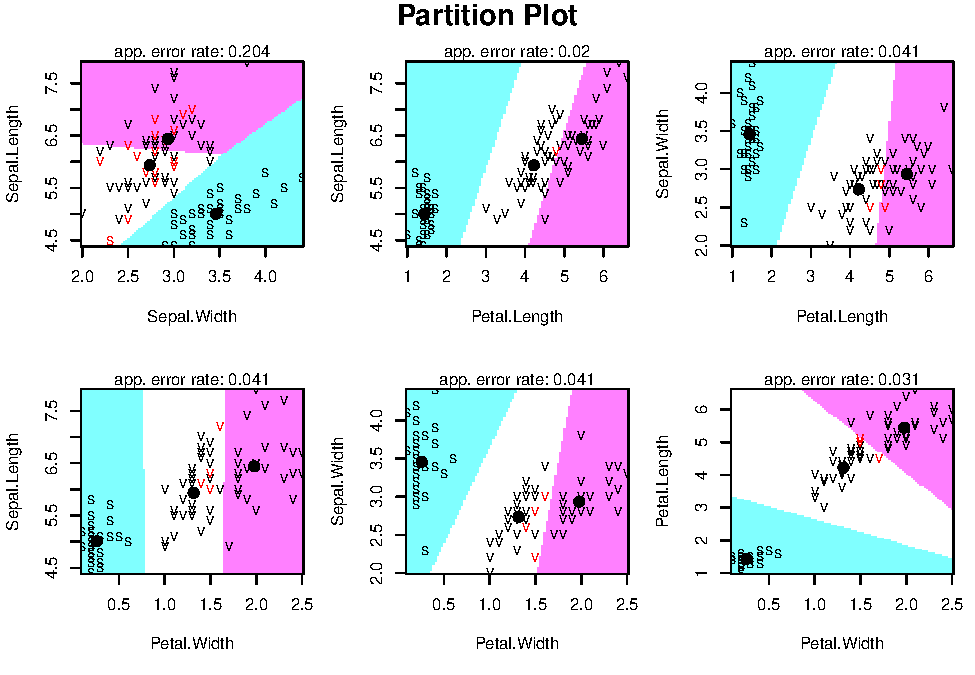
\includegraphics{LDA_QDA_IRIS_files/figure-latex/unnamed-chunk-4-1.pdf}

\begin{Shaded}
\begin{Highlighting}[]
\DocumentationTok{\#\#\# Confusion matrix and accuracy – training data}
\NormalTok{p1 }\OtherTok{=} \FunctionTok{predict}\NormalTok{(iris\_lda, training)}\SpecialCharTok{$}\NormalTok{class}
\NormalTok{tab }\OtherTok{=} \FunctionTok{table}\NormalTok{(}\AttributeTok{Predicted =}\NormalTok{ p1, }\AttributeTok{Actual =}\NormalTok{ training}\SpecialCharTok{$}\NormalTok{Species)}
\NormalTok{tab}
\end{Highlighting}
\end{Shaded}

\begin{verbatim}
##             Actual
## Predicted    setosa versicolor virginica
##   setosa         33          0         0
##   versicolor      0         34         0
##   virginica       0          0        31
\end{verbatim}

\hypertarget{predicting-the-classes-in-testing-set-based-on-the-lda-fit}{%
\section{Predicting the classes (In Testing Set) based on the LDA
fit}\label{predicting-the-classes-in-testing-set-based-on-the-lda-fit}}

\begin{Shaded}
\begin{Highlighting}[]
\NormalTok{p2 }\OtherTok{=} \FunctionTok{predict}\NormalTok{(iris\_lda, testing)}\SpecialCharTok{$}\NormalTok{class}
\NormalTok{tab1 }\OtherTok{=} \FunctionTok{table}\NormalTok{(}\AttributeTok{Predicted =}\NormalTok{ p2, }\AttributeTok{Actual =}\NormalTok{ testing}\SpecialCharTok{$}\NormalTok{Species)}
\NormalTok{tab1}
\end{Highlighting}
\end{Shaded}

\begin{verbatim}
##             Actual
## Predicted    setosa versicolor virginica
##   setosa         17          0         0
##   versicolor      0         14         0
##   virginica       0          2        19
\end{verbatim}

\hypertarget{qda-quadratic-discriminant-analysis-on-the-iris-data}{%
\section{QDA (Quadratic discriminant analysis on the IRIS
Data)}\label{qda-quadratic-discriminant-analysis-on-the-iris-data}}

\begin{Shaded}
\begin{Highlighting}[]
\DocumentationTok{\#\#Everything is not linear – quadratic discriminant analysis}

\NormalTok{iris\_qda}\OtherTok{=}\FunctionTok{qda}\NormalTok{(Species}\SpecialCharTok{\textasciitilde{}}\NormalTok{.,}\AttributeTok{data=}\NormalTok{training)}
\NormalTok{iris\_qda}
\end{Highlighting}
\end{Shaded}

\begin{verbatim}
## Call:
## qda(Species ~ ., data = training)
## 
## Prior probabilities of groups:
##     setosa versicolor  virginica 
##  0.3367347  0.3469388  0.3163265 
## 
## Group means:
##            Sepal.Length Sepal.Width Petal.Length Petal.Width
## setosa         5.006061    3.457576     1.439394   0.2575758
## versicolor     5.932353    2.735294     4.223529   1.3147059
## virginica      6.438710    2.935484     5.445161   1.9774194
\end{verbatim}

\begin{Shaded}
\begin{Highlighting}[]
\FunctionTok{summary}\NormalTok{(iris\_qda)}
\end{Highlighting}
\end{Shaded}

\begin{verbatim}
##         Length Class  Mode     
## prior    3     -none- numeric  
## counts   3     -none- numeric  
## means   12     -none- numeric  
## scaling 48     -none- numeric  
## ldet     3     -none- numeric  
## lev      3     -none- character
## N        1     -none- numeric  
## call     3     -none- call     
## terms    3     terms  call     
## xlevels  0     -none- list
\end{verbatim}

\begin{Shaded}
\begin{Highlighting}[]
\CommentTok{\#library(klaR)}
\FunctionTok{partimat}\NormalTok{(Species}\SpecialCharTok{\textasciitilde{}}\NormalTok{.,}\AttributeTok{data=}\NormalTok{training,}\AttributeTok{method=}\StringTok{"lda"}\NormalTok{)}
\end{Highlighting}
\end{Shaded}

\includegraphics{LDA_QDA_IRIS_files/figure-latex/unnamed-chunk-6-1.pdf}

\begin{Shaded}
\begin{Highlighting}[]
\FunctionTok{partimat}\NormalTok{(Species}\SpecialCharTok{\textasciitilde{}}\NormalTok{.,}\AttributeTok{data=}\NormalTok{training,}\AttributeTok{method=}\StringTok{"qda"}\NormalTok{)}
\end{Highlighting}
\end{Shaded}

\includegraphics{LDA_QDA_IRIS_files/figure-latex/unnamed-chunk-6-2.pdf}

\hypertarget{check-the-accuracy-of-our-analysis-of-qda-in-training-set}{%
\subsection{Check the accuracy of our analysis of QDA in Training
Set}\label{check-the-accuracy-of-our-analysis-of-qda-in-training-set}}

\begin{Shaded}
\begin{Highlighting}[]
\CommentTok{\#Check the accuracy of our analysis of qda}
\NormalTok{Predictions\_qda}\OtherTok{=}\FunctionTok{predict}\NormalTok{(iris\_qda,training)}
\FunctionTok{table}\NormalTok{(Predictions\_qda}\SpecialCharTok{$}\NormalTok{class, training}\SpecialCharTok{$}\NormalTok{Species)}
\end{Highlighting}
\end{Shaded}

\begin{verbatim}
##             
##              setosa versicolor virginica
##   setosa         33          0         0
##   versicolor      0         34         0
##   virginica       0          0        31
\end{verbatim}

\hypertarget{check-the-accuracy-of-our-analysis-of-qda-in-testing-set}{%
\subsection{\#\# Check the accuracy of our analysis of QDA in Testing
Set}\label{check-the-accuracy-of-our-analysis-of-qda-in-testing-set}}

\begin{Shaded}
\begin{Highlighting}[]
\CommentTok{\#Check the accuracy of our analysis of qda}
\NormalTok{Predictions\_qda}\OtherTok{=}\FunctionTok{predict}\NormalTok{(iris\_qda,testing)}
\FunctionTok{table}\NormalTok{(Predictions\_qda}\SpecialCharTok{$}\NormalTok{class, testing}\SpecialCharTok{$}\NormalTok{Species)}
\end{Highlighting}
\end{Shaded}

\begin{verbatim}
##             
##              setosa versicolor virginica
##   setosa         17          0         0
##   versicolor      0         14         0
##   virginica       0          2        19
\end{verbatim}

\end{document}
